\documentclass[10pt]{article}
\usepackage[ngerman]{babel}
\usepackage[utf8]{inputenc}
\usepackage[T1]{fontenc}
\usepackage{amsmath}
\usepackage{amsfonts}
\usepackage{amssymb}
\usepackage[version=4]{mhchem}
\usepackage{stmaryrd}
\usepackage{graphicx}
\usepackage[export]{adjustbox}
\graphicspath{ {./images/} }

\title{Hauptprüfung Abiturprüfung 2023 - Leistungsfach }

\author{Alexander Schwarz\\
www.mathe-aufgaben.com}
\date{}


\begin{document}
\maketitle
 Baden-Württemberg

\section*{Aufgabe C2}
Michael und Torsten spielen mit den beiden Würfeln, deren Netze abgebildet sind, folgendes Spiel: Michael würfelt mit dem Würfel $W_{1}$, Torsten würfelt mit dem Würfel $\mathrm{W}_{2}$. Der Spieler mit der höheren Augenzahl\\
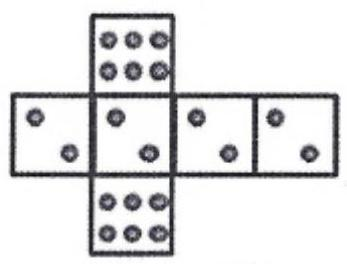
\includegraphics[max width=\textwidth, center]{2025_04_24_f1d48d7aff82ca38eaeag-2(1)}
Folgender Teil ist für die Aufgaben e und f.
Torsten hat den Verdacht, dass beim Würfel $W_{2}$ die Wahrscheinlichkeit für die Augenzahl 5 nicht $\frac{2}{3}$ beträgt. Daher wird ein einseitiger Hypothesentest mit 500\\
Würfen auf dem Signifikanzniveau s durchgeführt. Dabei ergibt sich die Entscheidungsregel, dass die Nullhypothese genau dann abgelehnt wird, wenn weniger als 318-mal die Augenzahl 5 erzielt wird.\\

Netz von W 1\\
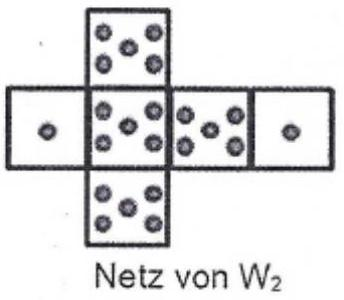
\includegraphics[max width=\textwidth]{2025_04_24_f1d48d7aff82ca38eaeag-2} gewinnt.\\
a) Geben Sie alle möglichen Würfelergebnisse an, bei denen Michael das Spiel gewinnt.\\
Begründen Sie, dass Michaels Gewinnwahrscheinlichkeit $\frac{5}{9}$ beträgt. (1 VP)\\
b) Michael und Torsten spielen 30 Spiele. Berechnen Sie die Wahrscheinlichkeit der folgenden Ereignisse:\\
A: „Michael gewinnt mindestens 13, aber höchstens 20 Spiele." (1 VP)\\
B: „Torsten gewinnt mehr Spiele als Michael."\\
c) Es werden n Spiele gespielt. Die Wahrscheinlichkeit dafür, dass Michael dabei nur das letzte Spiel gewinnt, soll weniger als 5\% betragen. Bestimmen Sie den kleinstmöglichen Wert von $n$.\\
(2 VP)\\
d) Das Spiel wird folgendermaßen verändert: Vor dem Würfeln wird ein Glücksrad mit einem grünen und einem roten Sektor einmal gedreht. Wenn dabei grün erscheint, dann behalten Michael und Torsten ihre Würfel: erscheint rot, dann tauschen sie die Würfel. Die Wahrscheinlichkeit dafür, dass Michael bei diesem Spiel eine höhere Zahl als Torsten würfelt, beträgt $\frac{7}{15}$. Bestimmen Sie für den grünen Sektor die Größe des Mittelpunktswinkels.\\
(2,5 VP)

e) Formulieren Sie die zugehörige Nullhypothese. Bestimmen Sie alle ganzzahligen Prozentwerte, die für s in Frage kommen.\\
f) Formulieren Sie den Fehler zweiter Art im Sachzusammenhang. (1 VP) Bestimmen Sie die Wahrscheinlichkeit für den Fehler zweiter Art unter der Annahme, dass beim Würfel $\mathrm{W}_{2}$ die Augenzahl 5 mit einer Wahrscheinlichkeit von 60\% erzielt wird.

\section*{Lösungen}
\section*{Aufgabe C2}
a) Geben Sie alle möglichen Würfelergebnisse an, bei denen Michael das Spiel gewinnt.

Die möglichen Würfelergebnisse sind: $(2 ; 1),(6 ; 1)$, $(6 ; 5)$\\
Begründen Sie, dass Michaels Gewinnwahrscheinlichkeit $\frac{5}{9}$ beträgt.\\
$P((2 ; 1))+P((6 ; 1))+P((6 ; 5))=\frac{2}{3} \cdot \frac{1}{3}+\frac{1}{3} \cdot \frac{1}{3}+\frac{1}{3} \cdot \frac{2}{3}=\frac{5}{9}$\\
b) Berechnen Sie die Wahrscheinlichkeit der folgenden Ereignisse

Die Zufallsgröße X sei die Anzahl der Spiele, die Michael gewinnt.\\
$X$ ist binomialverteilt mit $n=30$ und $p=\frac{5}{9}$.\\
$P(A)=P(13 \leq X \leq 20)=P(X \leq 20)-P(X \leq 12) \approx 0,922-0,063=0,859$\\
Ereignis B: Wenn Torsten mehr Spiele gewinnt als Michael, darf Michael maximal 14 Spiele gewinnen.\\
$\mathrm{P}(\mathrm{B})=\mathrm{P}(\mathrm{X} \leq 14) \approx 0,213$\\
c) Bestimmen Sie den kleinstmöglichen Wert von n.

Die Wahrscheinlichkeit, dass Michael die ersten n-1 Spiele verliert und das letzte Spiel gewinnt beträgt $\left(\frac{4}{9}\right)^{n-1} \cdot \frac{5}{9}$.\\
Bedingung: $\left(\frac{4}{9}\right)^{n-1} \cdot \frac{5}{9}<0,05$\\
Ausprobieren mit dem Taschenrechner:\\
$\left(\frac{4}{9}\right)^{2} \cdot \frac{5}{9} \approx 0,11>0,05$\\
$\left(\frac{4}{9}\right)^{3} \cdot \frac{5}{9} \approx 0,049<0,05$\\
Es gilt $\mathrm{n}-1=3 \Leftrightarrow \mathrm{n}=4$.\\
Somit müssen mindestens 4 Spiele gespielt werden.\\
d) Bestimmen Sie für den grünen Sektor die Größe des Mittelpunktswinkels.

Zur Berechnung des Mittelpunktswinkels muss zunächst die Wahrscheinlichkeit p berechnet werden, dass der grüne Sektor gedreht wird.\\
Der rote Sektor wird mit Wahrscheinlichkeit 1 - p gedreht.\\
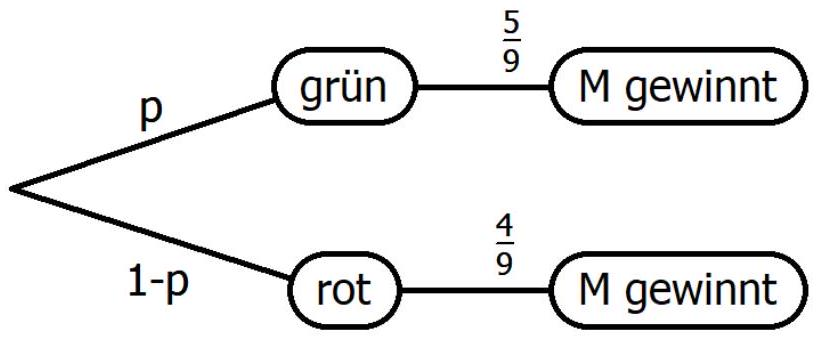
\includegraphics[max width=\textwidth, center]{2025_04_24_f1d48d7aff82ca38eaeag-4}\\
$P(M$ gewinnt $)=p \cdot \frac{5}{9}+(1-p) \cdot \frac{4}{9}=\frac{7}{15}$\\
$\Leftrightarrow \frac{1}{9} p+\frac{4}{9}=\frac{7}{15} \Leftrightarrow p=0,2$\\
Der Mittelpunktswinkel des grünen Sektors beträgt $360^{\circ} \cdot 0,2=72^{\circ}$.\\
e) Formulieren Sie die zugehörige Nullhypothese.

Der Ablehnungsbereich ist $\bar{A}=\{0,1,2, \ldots, 317\}$.\\
Aus diesem Ablehnungsbereich kann man erkennen, dass es sich um einen linksseitigen Hypothesentest handelt.\\
Es gilt $\mathrm{H}_{1}$ : $\mathrm{p}<\frac{2}{3}$\\
Daraus folgt $\mathrm{H}_{0}: \mathrm{p} \geq \frac{2}{3}$.

Hinweis: (Meinung des Autors)
Die Aufgabenstellung ist verwirrend gestellt.\\
Der Einleitungssatz der Aufgabe lautet:\\
„Torsten hat den Verdacht, dass beim Würfel $\mathrm{W}_{2}$ die Wahrscheinlichkeit für die Augenzahl 5 nicht $\frac{2}{3}$ beträgt."\\
Aus diesem Einleitungssatz kann man schließen, dass ein zweiseitiger Hypothesentest notwendig ist, da sich der Verdacht nicht auf eine konkrete Richtung bezieht. Korrekt wäre folgender Einleitungssatz gewesen:\\
„Torsten hat den Verdacht, dass beim Würfel $\mathrm{W}_{2}$ die Wahrscheinlichkeit für die Augenzahl 5 weniger als $\frac{2}{3}$ beträgt."

Bestimmen Sie alle ganzzahligen Prozentwerte, die für s in Frage kommen.\\
Die Zufallsgröße X gibt die Anzahl der Würfe an, bei denen eine 5 erzielt wird.\\
$X$ ist binomialverteilt mit $n=500$ und $p=\frac{2}{3}$.\\
$P(X$ liegt im Ablehnungsbereich $)=P(X \leq 317)=0,0673$\\
Außerdem gilt $P(X \leq 318)=0,0804$.\\
Das Signifikanzniveau gibt die maximale Wahrscheinlichkeit für einen Fehler 1.Art an. Dieses beträgt mindestens $6,73 \%$ und weniger als $8,04 \%$.\\
Somit kommen für das Signifikanzniveau s die Werte 7\% und 8\% in Betracht.\\
f) Formulieren Sie den Fehler zweiter Art im Sachzusammenhang.

Die Nullhypothese wird nicht abgelehnt, obwohl die Wahrscheinlichkeit eine 5 zu würfeln, kleiner als $\frac{2}{3}$ ist (das heißt dass die Gegenhypothese $H_{1}$ wahr ist).

Bestimmen Sie die Wahrscheinlichkeit für den Fehler zweiter Art unter der Annahme, dass beim Würfel $\mathrm{W}_{2}$ die Augenzahl 5 mit einer Wahrscheinlichkeit von 60\% erzielt wird.

Die Zufallsgröße X gibt die Anzahl der Würfe an, bei denen eine 5 erzielt wird. $X$ ist binomialverteilt mit $n=500$ und $p=0,6$.\\
$P($ Fehler 2. Art$)=\mathrm{P}(\mathrm{X}$ liegt nicht im Ablehnungsbereich $)$

$$
=P(X \geq 318)=1-P(X \leq 317) \approx 0,0545
$$

Die Wahrscheinlichkeit für einen Fehler 2.Art beträgt ca. 5,4\%.


\end{document}